\documentclass[../main.tex]{subfiles}

\begin{document}
%%%%%%%%%%%%%%%%%%%%%%%%%%%%%%%%%%%%%%%%%%%%%%%%%%%%
%                                                  %
% Differentialrechnung I -- Tangente und Ableitung %
%                                                  %
%%%%%%%%%%%%%%%%%%%%%%%%%%%%%%%%%%%%%%%%%%%%%%%%%%%%

\chapter{Differentialrechnung I -- Tangente und Ableitung}
\section{Die Sekante}
Steigung: $m = \frac{\Delta y}{\Delta x}$ \\ [7pt]
Wobei $\Delta x = x_1 - x_0$ und $\Delta y = y_1 - y_0$

\subsection{Sekante durch P und Q}
$P(x_0|f(x_0)), Q(x_1|f(x_1))$ auf dem Graphen $g(f)$ \\ [7pt]
Steigung der Sekante durch P und Q: \\ [7pt]
$m = \frac{f(x_1)-f(x_0)}{x_1 - x_0}$ \\ [7pt]
\textbf{Sekantengleichung (Punkt-Richtungs-Form)} \\ [7pt]
$(y - y_0) = m(x - x_0)$ \\ [7pt]
Steigung: $m = \frac{\Delta y}{\Delta x}$ = \textbf{Differenzquotient von f an der Stelle $x_0$}

\section{Tangente und Ableitung}
\subsection{Beispiel Quadratische Funktion}
Gegeben die Funktion (rot) $f(x) = x^2$. Gesucht der Differenzquotient von f an der Stelle $x_0$: \\
\begin{minipage}{0.5\textwidth}
    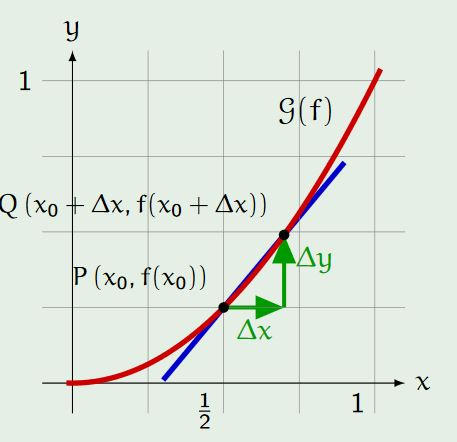
\includegraphics[width=50mm,scale=0.5]{tangente_example}
\end{minipage} \hfill
\begin{minipage}{0.45\textwidth}
    \begin{math}
        \frac{\Delta y}{\Delta x} = \frac{f(x_0 + \Delta x) - f(x_0)}{\Delta x} \\ [7pt]
        \frac{(x_0 + \Delta x)^2 - x_0^2}{\Delta x} \\ [7pt]
        \frac{x_0^2 + 2x_0\Delta x + \Delta x^2 - x_0^2}{\Delta x} \\ [7pt]
        \frac{2x_0\Delta x + \Delta x^2}{\Delta x} = 2x_0 + \Delta x \\ [7pt]
    \end{math}
    Steigung der Sekante : $2x_0 + \Delta x$ \\ [7pt]
    Gleichung der Sekante: \\ 
    $y = x_0^2 + (2x_0 + \Delta x)(x - x_0) = (2x_0 + \Delta x)x - (x_0 + \Delta x)x_0$. \\ [7pt]
\end{minipage}
Für die Tangente an der Stelle $x_0$ geht man mit dem Punkt Q immer näher an Punkt P, bis $\Delta x = 0$ (Weil die Tangente f nur an einer Stelle berührt) \\ [7pt]
$\lim\limits_{\Delta x\to 0} \frac{\Delta y}{\Delta x} = \lim\limits_{\Delta x\to 0} 2x_0 + \Delta x = 2x_0 = $ Steigung der Tangente \\ [7pt]
Damit Gleichung der Tangente an f: \\ [7pt]
$(y - f(x_0)) = 2x_0(x - x_0)$ \\ [7pt]
$y = f(x_0) + 2x_0(x - x_0) = x_0^2 + 2x_0(x - x_0) = 2x_0x - x_0^2$

\section{Ableitung der Potenzfunktion}
$f(x) = x^n$ \\ [7pt]
$f'(x) = nx^{n-1}$
\subsection{Beispiel Tangente}
Tangente $t(x)$ an der Stelle $P(1,1)$ an der Kurve $f(x)=x^2$? \\ [7pt]
$f(x)=x^2$, $f'(x)=2x$ \\ [7pt]
$P(1,1)$, $P(x_0/f(x_0))$ \\ [7pt]
$f'(x_0) = 2x_0 = 2 \times 1 = 2$ = Steigung Tangente \\ [7pt]
$t(x) = f(x_0) + f'(x_0) \times (x - x_0)$ \\ [7pt]
$= 1 + 2(x - 1) = 1 + 2x -2 = 2x -1$

\subsection{Newton-Raphson Verfahren}
Wir wollen die (nichtlineare) Gleichung $f(x) = 0$ lösen, dh wir wollen ein $x_*$ so finden, dass $f(x_*) = 0$. Idee: Starte mit $x_0$, und berechne den Schnittpunkt $x_1$ der Tangente durch $(x_0,f(x_0))$ mit der x-Achse. Wiederhole diesen Schritt! \\
\begin{minipage}{0.5\textwidth}
    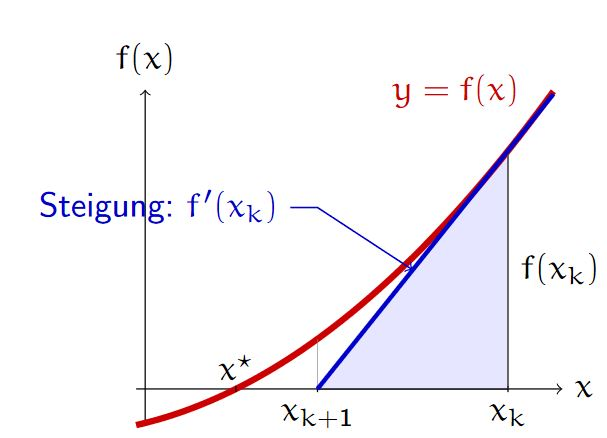
\includegraphics[width=50mm,scale=0.5]{newton_raphson_verfahren}
\end{minipage} \hfill
\begin{minipage}{0.45\textwidth}
    $f'(x_k) = \frac{f(x_k)}{x_k - x_{k+1}} = \frac{x_k}{-\Delta x_k}$ \\ [7pt]
    Ausgehend von $x_0$, iterieren wir über $k = 1,2,...$ \\ [7pt]
    $f'(x_k)\Delta x_k = -f(x_k)$
\end{minipage}
$x_{k+1} = x_k + \Delta x_k = x_k - [f'(x_k)]^-1f(x_k)$

\section{Einige Ableitungsregeln}
\subsection{Theorem Faktorregel}
Falls $f'(x)$ existiert, dann darf ein konstanter Faktor $c \in \mathbb{R}$ vor die Ableitung gezogen werden. \\ [7pt]
$[c \times f(x)]' = c \times f'(x)$ auch geschrieben als $\frac{d}{dx}[c \times f(x)] = c \times \frac{d}{dx}[f(x)]$

\subsection{Theorem Produkteregel}
Existieren die Ableitungen $u'(x)$ und $v'(x)$, dann gilt für die Ableitungen des Produkts die Regel: \\ [7pt]
$[u(x) \times v(x)]' = u'(x)v(x) + u(x)v'(x)$ \\ [7pt]
auch geschrieben als \\ [7pt]
$\frac{d}{dx}(u(x)v(x))=\frac{d}{dx}[u(x)]v(x) + u(x) \times \frac{d}{dx}[v(x)]$

\section{Quotientenregel}
Existieren die Ableitungen $u'(x)$ und $v'(x)$, dann gilt für die Ableitungen des Quotienten von $u(x)$ und $v(x) \neq 0$ die Regel: \\ [7pt]
$[\frac{u(x)}{v(x)}]' = \frac{u'(x)v(x) - u(x)v'(x)}{(v(x))^2}$ kurz $[\frac{u}{v}]'=\frac{u'v - uv'}{v^2}$ \\ [7pt]
auch geschrieben als \\ [7pt]
$\frac{d}{dx}[\frac{u(x)}{v(x)}] = \frac{\frac{d}{dx}[u(x)]v(x) - u(x) \frac{d}{dx} v(x)}{(v(x))^2}$ kurz $[\frac{u}{v}]'=\frac{u'v - uv'}{v^2}$



\section{Formeln}
Steigung: $m = \frac{\Delta y}{\Delta x}$ \\ [7pt]
Tangenten Gleichung: $t(x) = f(x_0) + f'(x_0) \times (x - x_0)$ \\ [7pt]
Faktorregel: $[c \times f(x)]' = c \times f'(x)$ \\ [7pt]
Produkteregel: $[u(x) \times v(x)]' = u'(x)v(x) + u(x)v'(x)$ \\ [7pt]
Quotientenregel: $[\frac{u(x)}{v(x)}]' = \frac{u'(x)v(x) - u(x)v'(x)}{(v(x))^2}$ kurz $[\frac{u}{v}]'=\frac{u'v - uv'}{v^2}$

\subsection{Ableitungen}
\label{sec:Ableitungen}
\begin{tabularx}{0.5\textwidth} { 
    >{\centering\arraybackslash}X 
    >{\centering\arraybackslash}X  }
    \hline
    f(x) & f'(x) \\ [7pt]
    \hline
    $x^n$ & $nx^{n-1}$
    \\ [7pt]
    $\sin(x)$ & $\cos(x)$
    \\ [7pt]
    $\cos(x)$ & $-\sin(x)$
    \\ [7pt]
    $\tan(x)$ & $\frac{1}{\cos^2(x)}$
    \\ [7pt]
    $e^x$ & $e^x$
    \\ [7pt]
    $e^{3x}$ & $3e^{3x}$
    \\ [7pt]
    $c (c \in \mathbb{R})$ & $0$
    \\ [7pt]
    $x$ & $1$
    \\ [7pt]
    $\sum\limits_{k=0}^n c_kx^k$ & $\sum\limits_{k=0}^n c_kx^{k-1}$
\end{tabularx}




\end{document}